\chapter{Optimización del proceso de valoración de puntos de interés}

	\section{Clasificación de imágenes mediante redes convolucionales}
	
		Una primera aproximación a agilizar el proceso de valoración comentado, sería detectar el objeto que se muestra en la imagen de la propuesta, para que en caso de que sea algo aceptable proseguir con el proceso de valoración, o en caso contrario, rechazar directamente la propuesta. Para comenzar este caso práctico, lo primero a realizar es el proceso conocido como ETL, que consiste en la extracción, transformación, y carga de los datos; para posteriormente poder trabajar con ellos y proporcionárselos al modelo. Comenzando por la extracción de datos, se presenta el primero de los problemas. La idea es utilizar imágenes que realmente hayan pasado por este proceso de valoración para poder hacer el proyecto lo más realista posible, sin embargo, ni Wayfarer ni ninguno de los juegos poseen alguna API (al menos de manera pública) que permita recolectar de manera programática las imágenes utilizadas o información relativa a ellas. 
		
		\subsection{Proceso ETL}
		
			La solución adoptada para este proceso, ha sido recolectar manualmente imágenes que han superado el proceso de valoración, pudiendo consultar algunas de ellas desde el mapa de uno de los juegos (\url{https://intel.ingress.com/}). En este caso, se estarían clasificando entre las $n$ clases de objetos aceptables las imágenes recibidas, cosa que en un primer momento parece carecer de sentido pues se conoce el resultado de la valoración. Sin embargo, al no tener acceso a propuestas rechazadas, no se pueden recolectar estos datos para entrenar los modelos, pero si de la empresa responsable se tratase, se dispondría de una enorme cantidad de imágenes válidas y no válidas etiquetadas, y que se podrían cargar de manera automática. En resumen, cambiando simplemente los datos que se cargarían y su fuente, se podrían tomar las siguientes decisiones sin necesidad de modificar el resto del proyecto.  
			
			\begin{itemize}
				\item Si $I \in C_i, 0 \leq i < m$, rechazar la propuesta
				\item Si $I \in C_j, m \leq j < n$, continuar evaluando la propuesta
			\end{itemize}
			
			Continuando con la extracción de los datos, y preparándolos para la carga, se ha creado una carpeta \texttt{tfg\_dataset} que representa el conjunto de las imágenes que se utilizan durante el proyecto. Dentro de esta, se ubicarán dos subcarpetas, \texttt{train} y \texttt{test}, que hacen referencia a las imágenes que se utilizarán para entrenar los modelos, y las que se utilizarán para evaluar su rendimiento. Dentro de cada una de esas carpetas deberán crearse subcarpetas donde se encuentren las imágenes separadas por sus clases, siendo esta la manera de etiquetar el conjunto de datos y prepararlo para la carga. Se puede visualizar un breve esquema de esta estructura en la \Cref{fig:arbol_dataset}. \\
			
			\begin{figure}[!h]
				\centering
				\Tree[.\texttt{tfg\_dataset} [.\texttt{train} \texttt{clase\_1} \texttt{clase\_2} \texttt{clase\_3} $\cdots$ ] [.\texttt{test} \texttt{clase\_1} \texttt{clase\_2} \texttt{clase\_3} $\cdots$ ] ]
				\caption{Árbol de carpetas del dataset}
				\label{fig:arbol_dataset}
			\end{figure}
			
			Para cargar el dataset en TensorFlow directamente desde la estructura de carpetas creadas, se hará uso de la función \texttt{image\_dataset\_from\_directory} del paquete \texttt{utils}. Esta contiene una serie de parámetros interesantes a comentar. 
			
			\begin{itemize}
				\item \texttt{directory}: es el directorio raíz del dataset, en este caso \texttt{tfg\_dataset}. 
				\item \texttt{image\_size}: es una tupla de dos elementos con las dimensiones en píxeles que deberán tener las imágenes del dataset. 
				\item \texttt{labels}: mediante el valor \texttt{inferred} las etiquetas toman el mismo valor que el nombre de las carpetas. 
				\item \texttt{label\_mode}: hace referencia a la forma de codificar las etiquetas. Se empleará el valor \texttt{categorical} para codificar las etiquetas utilizando one-hot-encoding, es decir, si se tienen por ejemplo cuatro clases y un elemento pertenece a la cuarta, dicha etiqueta queda codificada como 0001. 
				\item \texttt{batch\_size}: hace referencia al tamaño de batch o lote que será utilizado durante el entrenamiento. Si en la función de entrenamiento se elige un tamaño diferente, se utilizará el menor de los valores. 
				\item \texttt{validation\_split}: hace referencia al porcentaje de los datos de entrenamiento que se reservan para validar el modelo durante el entrenamiento, es decir, permiten calcular el error del modelo al hacer una predicción de datos que nunca ha visto mientras entrena. Se reservarán un 20\% de los datos para validar. 
				\item \texttt{seed}: hace referencia a la semilla que se utiliza para ordenar las imágenes de manera aleatoria. 
				\item \texttt{subset}: seleccionando el valor \texttt{both} permite devolver el conjunto de entrenamiento y validación con la llamada a la función, es decir, \texttt{x\_train, x\_val = image\_dataset\_from\_directory(...)}. 
			\end{itemize}
			
			Como se puede observar, esta función que está haciendo principalmente el trabajo de la carga de datos, también hace parte del proceso de transformación, ya que permite modificar las dimensiones de la imagen, en este caso se utilizará un valor de $224 \times 224$ píxeles. Además, cada píxel (en cada canal de color) toma un valor entre 0 y 255. Es muy importante normalizar estos valores en el proceso de transformación para facilitar el trabajo a los diferentes modelos. Para ello, con ayuda de una capa de reescalado de Keras, se divide el valor de cada píxel entre 255 para obtener valores entre 0 y 1. Con motivo de verificar que todos estos pasos se han realizado correctamente, se codificado una función llamada \texttt{sample\_ds\_dfd} que permite visualizar nueve ejemplos aleatorios de un dataset creado con la función de TensorFlow mencionada, obteniendo como resultado la \Cref{fig:sample_dataset}. \\
			
			\begin{figure}
				\centering
				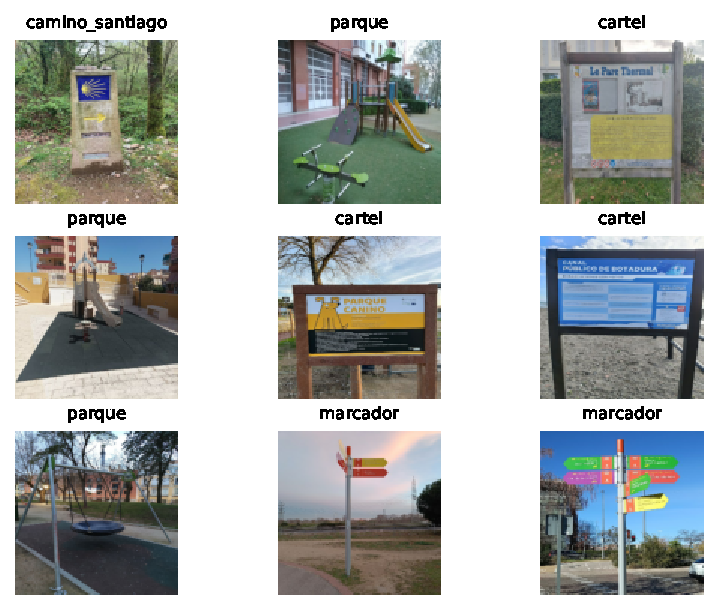
\includegraphics[scale = .8]{sample_dataset}
				\caption{Visualización de ejemplo de un dataset creado}
				\label{fig:sample_dataset}
			\end{figure}
			
		\subsection{Creación y entrenamiento de una red convolucional en TensorFlow}\label{subsec:crear_cnn}
		
			En esta primera aproximación se va a crear y entrenar una red convolucional desde cero con el dataset mencionado. Mediante la clase \texttt{Sequential} de Keras, se puede proporcionar una lista de las capas que conforman el modelo. La primera de ellas será una capa de convolución, con la particularidad de que se debe indicar el tamaño de entrada, siendo este un tensor de las dimensiones indicadas en la creación del dataset. Se alterna cada capa de convolución ReLU de stride $3 \times 3$ y 32 o 64 filtros, con una capa de maxpooling con stride $2 \times 2$. Estos valores han sido elegidos de manera arbitraria. Esta arquitectura se puede visualizar en la \Cref{fig:arq_cnn}. \\
			
			\begin{figure}[!h]
				\centering
				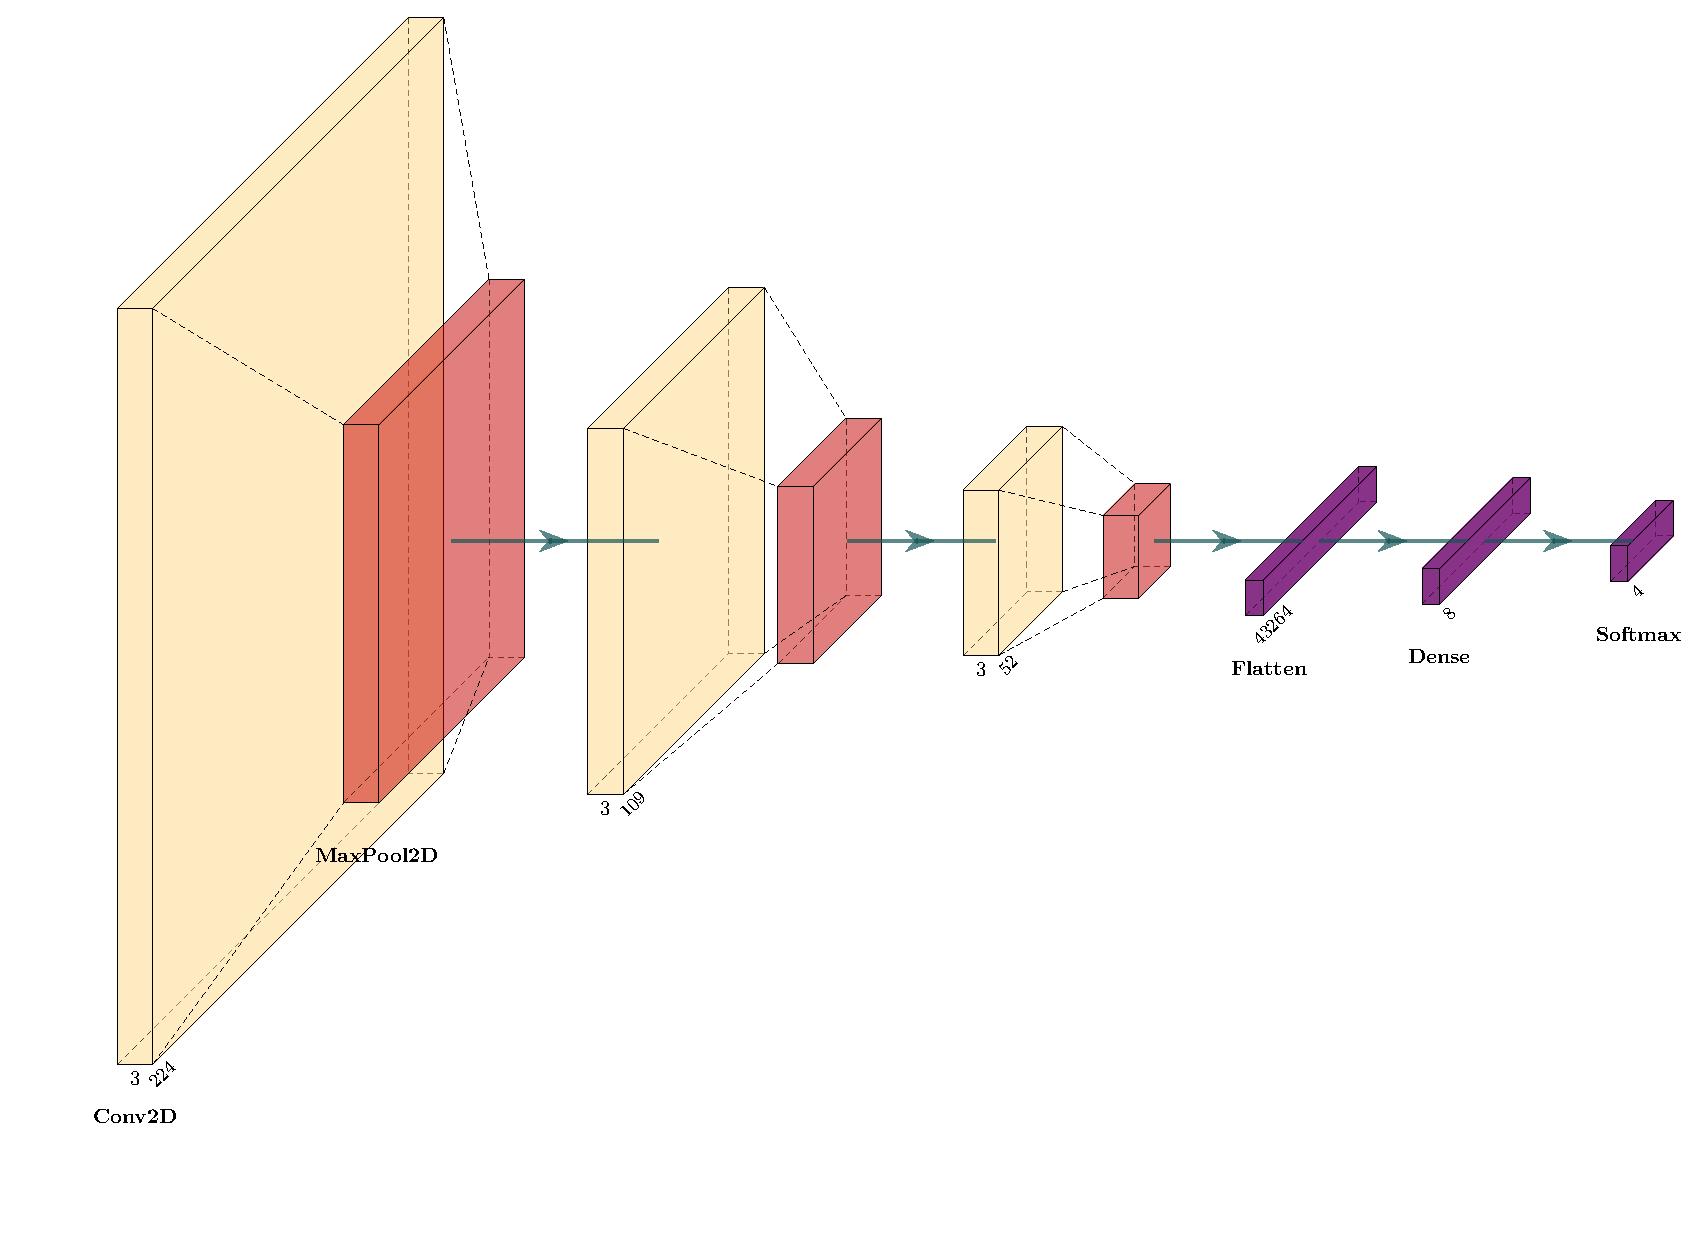
\includegraphics[scale = .55]{arq_cnn}
				\caption{Arquitectura de la red convolucional}
				\label{fig:arq_cnn}
			\end{figure}
			
			Mediante estas capas, se supone que la red debe extraer características de las imágenes, como por ejemplo
			
			\begin{itemize}
				\item Aparece un objeto rectangular
				\item Tiene dos patas 
				\item No tiene formas curvas
			\end{itemize}
			y de ahí con ayuda de una red clásica, ser capaz de deducir que en la imagen aparece un cartel. En realidad, las capas de convolución no obtienen características tan claras, pero sí resultan con una matriz de detalles en la imagen que pueden conducir a la misma conclusión. Para ello se utiliza la capa \texttt{Flatten} que transforma dicha matriz en un vector que sirve de entrada a la siguiente y última capa de la red, una capa oculta con tantas neuronas como clases diferentes. Como función de activación se utiliza softmax para obtener una distribución de probabilidad en la que se observe cuál es claramente la clase a la que pertenece el objeto, y con qué confianza lo es. Finalmente, mediante la función \texttt{summary} se puede observar un resumen del modelo. 
			
			\begin{verbatim}
				_________________________________________________________________
				Layer (type)                Output Shape              Param #   
				=================================================================
				conv2d (Conv2D)             (None, 222, 222, 32)      896       
				
				max_pooling2d (MaxPooling2  (None, 111, 111, 32)      0         
				D)                                                              
				
				conv2d_1 (Conv2D)           (None, 109, 109, 64)      18496     
				
				max_pooling2d_1 (MaxPoolin  (None, 54, 54, 64)        0         
				g2D)                                                            
				
				conv2d_2 (Conv2D)           (None, 52, 52, 64)        36928     
				
				max_pooling2d_2 (MaxPoolin  (None, 26, 26, 64)        0         
				g2D)                                                            
				
				flatten (Flatten)           (None, 43264)             0         
				
				dense_2 (Dense)             (None, 8)                 346120    
				
				dense_3 (Dense)             (None, 4)                 36        
				
				=================================================================
				Total params: 402476 (1.54 MB)
				Trainable params: 402476 (1.54 MB)
				Non-trainable params: 0 (0.00 Byte)
				_________________________________________________________________
			\end{verbatim}
			
			Con la función \texttt{compile} se termina de crear el objeto que representa al modelo, pudiendo especificar un optimizador, la función de pérdida, y las métricas que se muestran durante el entrenamiento. Para este proyecto se utilizarán Adam, entropía cruzada, y precisión respectivamente. El modelo ya está en condiciones de ser entrenado, y esto se logra mediante la función \texttt{fit}, a la que se le proporcionan los datos de entrenamiento (\texttt{x\_train}), los datos de validación (\texttt{x\_val}), el número de épocas (en este caso se han elegido 25), y la ruta de los callbacks. Esta sirve para ir almacenando metadatos del entrenamiento, que mediante una utilidad con la que cuenta TensorFlow llamada TensorBoard, permite monitorizar de manera muy visual la calidad del entrenamiento, tal y como se muestra en la \Cref{fig:tb_cnn}. \\
			
			\begin{figure}[!h]
				\centering
				\begin{subfigure}{.4\textwidth}
					\centering
					\includesvg[width = .85\textwidth]{evaluation_loss_vs_iterations_cnn}
					\caption{Iteraciones frente a pérdida}
					\label{fig:tb_cnn_a}
				\end{subfigure}\hfill
				\begin{subfigure}{.4\textwidth}
					\centering
					\includesvg[width = .85\textwidth]{evaluation_accuracy_vs_iterations_cnn}
					\caption{Iteraciones frente a precisión}
					\label{fig:tb_cnn_b}
				\end{subfigure}
				\begin{subfigure}{.4\textwidth}
					\centering
					\includesvg[width = .85\textwidth]{epoch_loss_cnn}
					\caption{Pérdida sobre el conjunto de entrenamiento y validación}
					\label{fig:tb_cnn_c}
				\end{subfigure}\hfill
				\begin{subfigure}{.4\textwidth}
					\centering
					\includesvg[width = .85\textwidth]{epoch_accuracy_cnn}
					\caption{Precisión sobre el conjunto de entrenamiento y validación}
					\label{fig:tb_cnn_d}
				\end{subfigure}
				\caption{Pérdida y precisión durante el entrenamiento de la CNN}
				\label{fig:tb_cnn}
			\end{figure}
			
			La situación que describen las gráficas, es negativa y sería la típica no deseada, pues se observa como con el paso de las iteraciones el error crece mientras que la precisión se estanca en valores no deseados. En concreto, en la \Cref{fig:tb_cnn_c} se observa cómo el error sobre el conjunto de validación crece, mientras que sobre el conjunto de entrenamiento tiende a cero. Esta es una situación denominada como sobreaprendizaje u \textit{overfitting}\cite{overfitting}. La red no tiene capacidad de aprender ni generalizar, y lo que está haciendo es memorizar los datos de ejemplo que se le presentan, cometiendo entonces errores cuando recibe datos que no ha visto nunca. 
			
		\subsection{Transfer learning en TensorFlow}
		
			Como se ha podido observar durante la sección anterior, el resultado del entrenamiento no ha sido adecuado, pues la red tendía a memorizar los datos que se le presentaban sin mostrar una buena capacidad de generalización. Esto puede deberse a múltiples factores, como por ejemplo, que al tener un conjunto de datos de entrenamiento tan reducido no sea capaz de extraer correctamente las características que determinan a los objetos de cada clase. Es decir, en vez de hacerle llegar a las capas densas hechos como ``tiene un objeto rectangular'', ``tiene dos patas'', etc; podría estar haciéndole llegar, ``hay dos árboles en el fondo''. Observando la estructura del modelo, se está tratando de optimizar cerca un millón de parámetros con poco más de 500 observaciones, algo que es muy desproporcionado; la red no es capaz de encontrar relaciones con tan pocos datos. \\
			
			En proyectos similares del mundo real, y en los que además se dispone de pocos datos (como es el caso), es muy poco frecuente crear y entrenar un modelo desde cero tal y como se ha realizado en la \Cref{subsec:crear_cnn}. En vez de realizar esto, es muy común utilizar una técnica conocida como transfer learning. Tal y como se menciona en \cite{transfer}, es una técnica muy aplicada en casos en los que se dispone de pocos datos y los modelos de deep learning no son capaces de encontrar relaciones, y también en casos en los que se dispone de equipos con pocos recursos. Consiste en aplicar el conocimiento obtenido de otro dataset, no necesariamente relacionado, para facilitar el proceso de obtener el conocimiento deseado del dataset actual. \\
			
			En el problema que se está tratando, se va a aplicar esta técnica de la siguiente manera. Como previamente se ha mencionado, las redes convolucionales, pueden verse como un conjunto de capas capaces de extraer características de las imágenes, junto con una red neuronal clásica que es capaz de clasificar en función de dichas características. Teniendo en cuenta que el principal problema del modelo anterior podría ser que no fuera capaz de obtener las características adecuadas que definen a cada clase, la idea es utilizar una serie de capas que sí sean capaces de obtener de manera correcta las características de una imagen, para después poder entrenar la red neuronal clásica con las características adecuadas. \\
			
			Con ayuda de la librería TensorHub que trabaja junto con TensorFlow, se pueden importar modelos ya entrenados de \url{https://www.kaggle.com/}. En este caso para aplicar la técnica de transfer learning, se ha decidido utilizar la red MobileNet de Google. El modelo se puede importar como si de una capa se tratase al crear un modelo secuencial de Keras. Para lograr la técnica, será clave declarar que los parámetros de dicha capa no se deberán entrenar (pues al importar el modelo ya vienen con unos valores adecuados). A continuación se coloca una capa densa, encargada de clasificar las características que la red de Google extraiga, y que deberá ser entrenada. Esta vez, el número de parámetros a optimizar sí es más adecuado al número de observaciones disponibles. 
			
			\begin{verbatim}
				_________________________________________________________________
				Layer (type)                Output Shape              Param #   
				=================================================================
				keras_layer (KerasLayer)    (None, 1280)              2257984   
				
				dense (Dense)               (None, 8)                 10248     
				
				dense_1 (Dense)             (None, 4)                 36        
				
				=================================================================
				Total params: 2268268 (8.65 MB)
				Trainable params: 10284 (40.17 KB)
				Non-trainable params: 2257984 (8.61 MB)
				_________________________________________________________________
			\end{verbatim}
			
			La manera de lanzar el entrenamiento es la misma que en el anterior, sin embargo, esta vez los resultados obtenidos son totalmente distintos, tal y como muestran las gráficas de TensorBoard en la \Cref{fig:tb_tl}. \\
			
			\begin{figure}[!h]
				\centering
				\begin{subfigure}{.4\textwidth}
					\centering
					\includesvg[width = .85\textwidth]{evaluation_loss_vs_iterations_mb}
					\caption{Iteraciones frente a pérdida}
					\label{fig:tb_tl_a}
				\end{subfigure}\hfill
				\begin{subfigure}{.4\textwidth}
					\centering
					\includesvg[width = .85\textwidth]{evaluation_accuracy_vs_iterations_mb}
					\caption{Iteraciones frente a precisión}
					\label{fig:tb_tl_b}
				\end{subfigure}
				\begin{subfigure}{.4\textwidth}
					\centering
					\includesvg[width = .85\textwidth]{epoch_loss_mb}
					\caption{Pérdida sobre el conjunto de entrenamiento y validación}
					\label{fig:tb_tl_c}
				\end{subfigure}\hfill
				\begin{subfigure}{.4\textwidth}
					\centering
					\includesvg[width = .85\textwidth]{epoch_accuracy_mb}
					\caption{Precisión sobre el conjunto de entrenamiento y validación}
					\label{fig:tb_tl_d}
				\end{subfigure}
				\caption{Pérdida y precisión durante el entrenamiento aplicando transfer learning}
				\label{fig:tb_tl}
			\end{figure}
			
			Estas gráficas representan una situación cercana a la ideal. En las \Cref{fig:tb_tl_a,fig:tb_tl_b} se observa cómo con el paso de las iteraciones, el error disminuye y la precisión aumenta hasta llegar a valores adecuados. Además, en las \Cref{fig:tb_tl_c,fig:tb_tl_d} se muestra claramente que tanto el error como la precisión se comportan de manera similar sobre los conjuntos de entrenamiento y validación respectivamente, tomando además valores adecuados. 
			
		\subsection{Aumento de datos}
		
			Como se ha visto a lo largo de las secciones anteriores, uno de los problemas que se está teniendo en este caso práctico, es la falta de datos. Una técnica utilizada frecuentemente en estos casos es conocida como aumento de datos. Consiste en modificar las imágenes del dataset de entrenamiento para que el modelo disponga de más ejemplos diferentes\cite{augm}. Podría entenderse como una parte del proceso de transformación ETL. \\
			
			Una vez más, es posible aplicar esta técnica mediante funciones de TensorFlow. Para ello se crea un objeto de la clase \texttt{ImageDataGenerator}. Mediante su constructor se pueden declarar los valores que toman los atributos que modificarán las imágenes, siendo algunos de los más destacables: 
			
			\begin{itemize}
				\item \texttt{rotation\_range}: gira la imagen. 
				\item \texttt{width\_shift\_range} y \texttt{height\_shift\_range}: desplazamiento horizontal y vertical de la imagen. 
				\item \texttt{shear\_range}: estira la imagen. 
				\item \texttt{zoom\_range}: hace zoom a la imagen. 
				\item \texttt{reescale}: indica el factor por el que se reescala la imagen, en este caso $1/255$ para facilitar el entrenamiento a la red, como en casos anteriores. 
				\item \texttt{validation\_split}: porcentaje de los datos reservados a validación. 
			\end{itemize}
			
			Una vez se tiene declarado el generador, se utiliza su método \texttt{flow\_from\_directory} para que dada la ruta que contiene las imágenes, el tamaño deseado de imagen, y el tamaño de los lotes, se cree el objeto que representa al dataset. De manera similar a la anterior, se ha programado una función \texttt{sample\_ds\_ffd} que permite visualizar nueve elementos del dataset creado, tal y como muestra la \Cref{fig:sample_dataset_au}. Esta es una de la manera más común de crear datos nuevos, siendo alguna de las más novedosas las arquitecturas GAN. Están formadas por dos redes, una capaz de crear imágenes y otra capaz de distinguir entre imágenes reales y generadas, y transmitir dicho conocimiento a la primera red, de manera que una intente ``engañar'' a la otra\cite{gan}. \\
			
			\begin{figure}
				\centering
				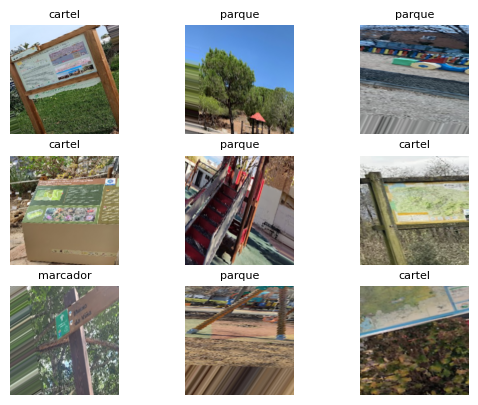
\includegraphics[scale = .8]{sample_dataset_au}
				\caption{Visualización de ejemplo de un dataset aplicando aumento de datos}
				\label{fig:sample_dataset_au}
			\end{figure}
			
			Contando ahora con el dataset original y el modificado, la técnica del aumento de datos se puede aplicar de dos formas. La primera de ellas es crear un modelo y entrenar únicamente con el datset modificado. Esto puede dar una mayor capacidad de generalización al modelo al mostrar imágenes más diferentes de objetos similares. La segunda de ellas consiste en entrenar el modelo con el dataset original, y después con el dataset modificado (sin cambiar qué imágenes pertenecen a los conjuntos de entrenamiento, validación, y test en cada dataset). Esta puede dar mejores resultados, pues tiene más observaciones y el modelo puede de ver el mismo objeto ``de diferentes formas''. Sin embargo hay que tener cuidado con esta segunda opción, pues podría conducir a situaciones de sobreajuste. 
			
		\subsection{Evaluación de los modelos}
		
			Si bien gracias a las gráficas que TensorBoard proporciona es posible hacerse una idea de la calidad que tendrán las predicciones de un modelo, no son suficientes. Será entonces el momento de presentar al modelo una serie de imágenes que nunca haya visto para poder evaluar la calidad de sus predicciones mediante una serie de métricas y valores estadísticos. Este conjunto de imágenes que el modelo no ha recibido hasta el momento, es el denominado conjunto de test. \\
			
			Para calcular estas métricas en Python, se va a utilizar la librería Scikit-learn, ya que contiene un conjunto de métodos con los que calcular y visualizar la mayoría de métricas empleadas en machine learning. Además, las predicciones sobre los conjuntos de test quedará representadas mediante dos matrices, \texttt{Y\_matrix} y \texttt{Y\_score}. La primera de ellas es una matriz $n \times 3$ que contiene para cada observación su etiqueta real, la predicha, y con qué probabilidad se le asigna. La segunda, contiene las probabilidades de cada observación de pertenecer a cada clase, por tanto es de dimensiones $n \times c$. 
			
			\begin{align*}
				Y_m &= \begin{pmatrix}
					0 & 0 & 0.75\\
					2 & 2 & 0.7\\
					3 & 1 & 0.97\\
					\vdots & \vdots & \vdots\\
					1 & 1 & 0.87
				\end{pmatrix} & 
				Y_s &= \begin{pmatrix}
					0.75 & 0.07 & 0.01 & 0.17\\
					0.15 & 0.01 & 0.7 & 0.14\\
					0.02 & 0.97 & 0.01 & 0.01\\
					\vdots & \vdots & \vdots & \vdots\\
					0.05 & 0.87 & 0.01 & 0.08
				\end{pmatrix}
			\end{align*}
			
			Dependiendo si el problema en cuestión es de regresión o clasificación, se deben utilizar unas métricas u otras. Debido a que se desea evaluar la calidad de una clasificación, se han elegido las siguientes. 
			
			\subsubsection{Matriz de confusión}
			
				La matriz de confusión muestra en el caso de clasificación binaria, los verdaderos positivos, verdaderos negativos, falsos positivos, y falsos negativos, mientras que en el caso de clasificación no binaria, en general la relación entre las etiquetas reales de cada observación y las que el modelo le ha asignado\cite{confusion}. De manera muy visual se puede observar la cantidad de ejemplos de cada clase (pudiendo ver si se encuentran desbalanceadas), cuántos han sido clasificados correctamente, cuántos no, y en general entre qué clases suele confundirse más el modelo. \\
				
				\begin{figure}[!h]
					\centering
					\begin{subfigure}{.4\textwidth}
						\centering
						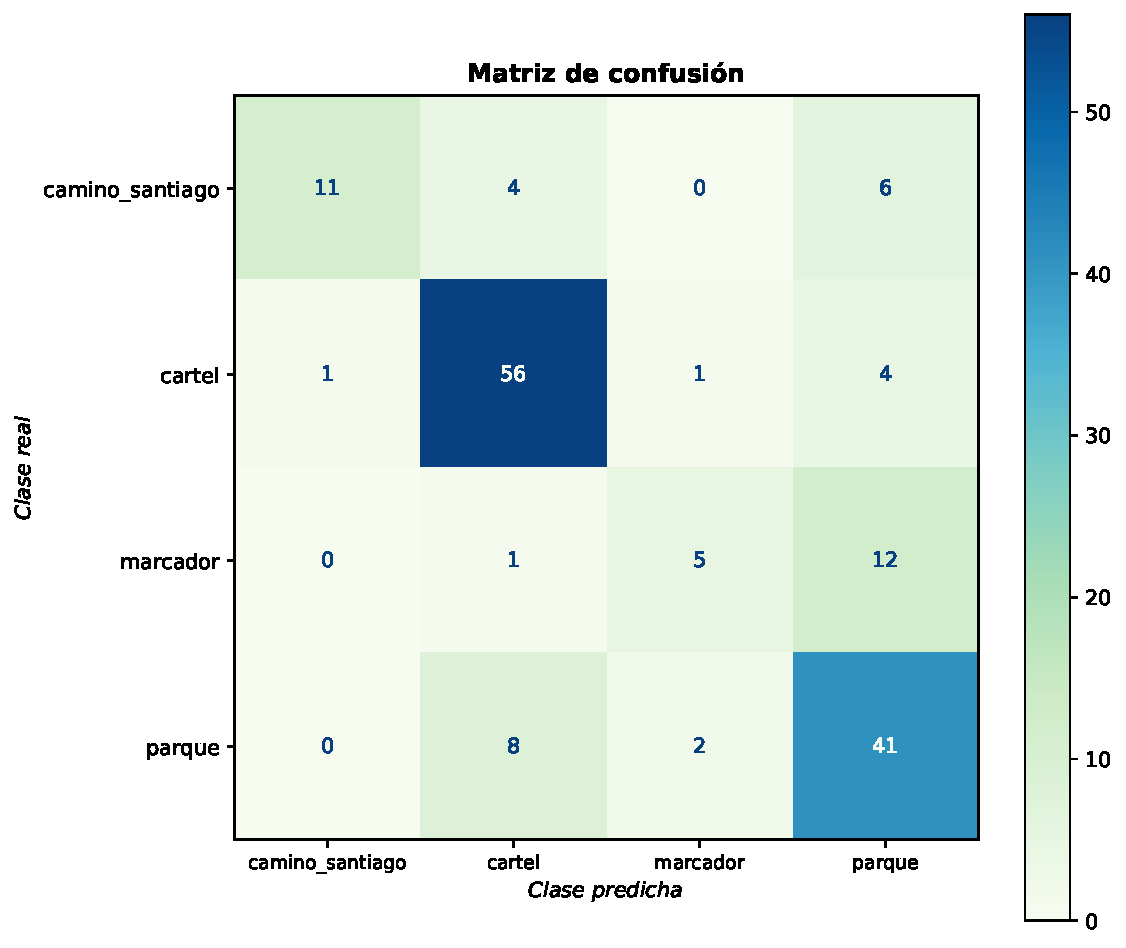
\includegraphics[scale = .42]{mc_conv}
						\caption{Normal}
						\label{fig:mc_conv}
					\end{subfigure}\hfill
					\begin{subfigure}{.4\textwidth}
						\centering
						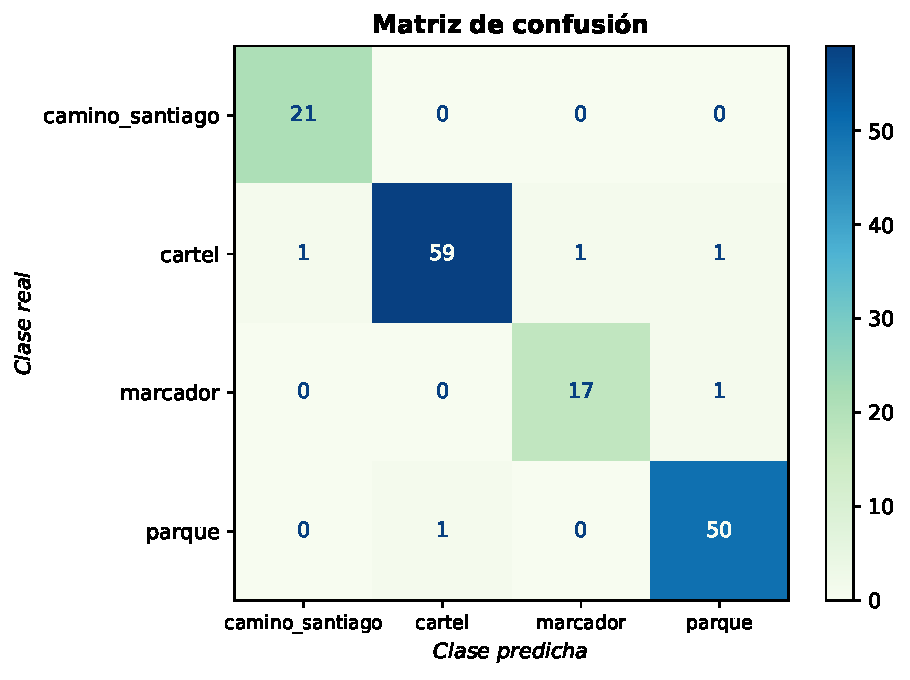
\includegraphics[scale = .42]{mc_mb}
						\caption{Aplicando transfer learning}
						\label{fig:mc_mb}
					\end{subfigure}
					\begin{subfigure}{.4\textwidth}
						\centering
						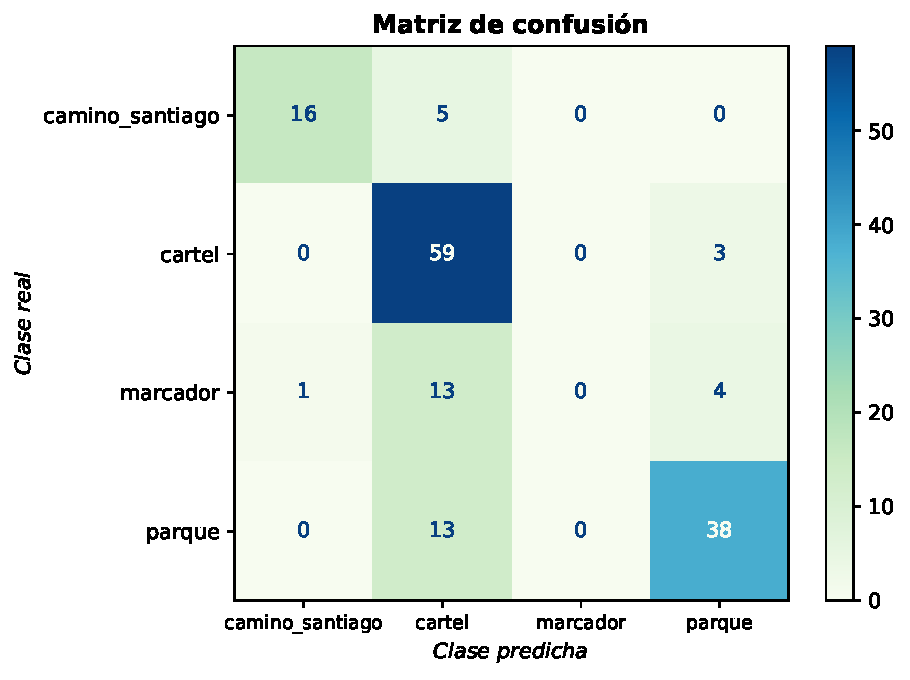
\includegraphics[scale = .42]{mc_convau}
						\caption{Aplicando aumento de datos}
						\label{fig:mc_convau}
					\end{subfigure}\hfill
					\begin{subfigure}{.4\textwidth}
						\centering
						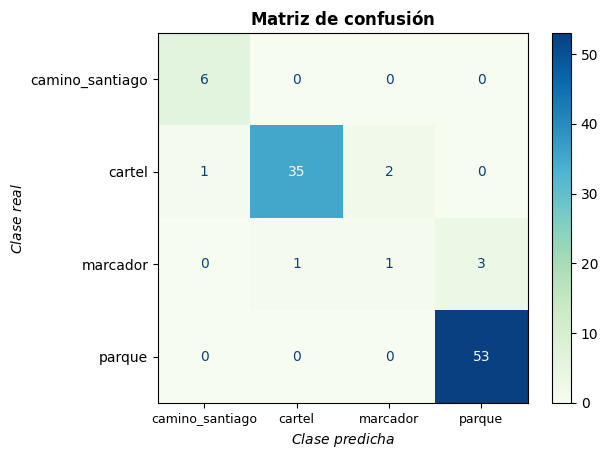
\includegraphics[scale = .42]{mc_mbau}
						\caption{Aplicando ambas}
						\label{fig:mc_mbau}
					\end{subfigure}
					\caption{Matrices de confusión}
					\label{fig:mc}
				\end{figure}
				
				En la \Cref{fig:mc} se observan las matrices de confusión de las cuatro situaciones descritas anteriormente. El elemento $a_{ij}$ representa la cantidad de observaciones de la clase $C_i$ que han sido clasificadas como $C_j$ (a partir de ahora, $\hat{C}_j$). La situación ideal se da cuando en el caso de que $i \neq j$, entonces $a_{ij} = 0$, o lo que es lo mismo, que solo haya valores  en la diagonal principal, pues a todos se les estaría asignando la clase correcta. Además, en esta representación gráfica sería deseable que todos los elementos de dicha diagonal tuviesen el mismo color, pues la situación actual describe un desbalanceo entre las clases. Se ve claramente que al aplicar transfer learning (\Cref{fig:mc_mb,fig:mc_mbau}) se obtienen resultados mucho mejores que al entrenar el modelo desde cero, tal y como las curvas de TensorBoard parecían indicar, pues la cantidad de malas clasificaciones es muy pequeña. La diferencia en dicho caso entre usar aumento de datos o no, no es muy significativa. \\
				
				Para poder calcular la matriz de confusión, se ha utilizado la función \texttt{confusion\_matrix} de Scikit-learn, que recibe como parámetros un vector con las clases reales de cada observación, y otro con las que el modelo les ha asignado. Mediante la función \texttt{ConfusionMatrixDisplay} se puede ver de manera gráfica la matriz (\Cref{fig:mc}). Con diferentes parámetros se pueden cambiar los colores e incrustar código \LaTeX{} para modificar los textos. Se ha codificado la función \texttt{matriz\_confusion} que recibe el dataset y $Y_m$, y muestra el gráfico con la configuración personalizada. 
				
			\subsubsection{Precisión, sensibilidad, y $F_1-$score}
				
				Si bien la matriz de confusión permite mostrar de manera visual la calidad de las clasificaciones, es conveniente calcular algunos valores \cite{metricas_matriz} a partir de esta matriz que permitan visualizar de manera numérica dichas calidades. La primera de ellas conocida como \textbf{precisión} $(\mathcal{P})$, y puede entenderse como la probabilidad de que un elemento que etiquetado como $C_i$, realmente pertenezca a dicha clase. 
				
				$$
				\mathcal{P} = P(C_i | \hat{C}_i) = \frac{P(C_i \cap \hat{C}_i)}{P(\hat{C}_i)}
				$$
				
				La siguiente se denomina \textbf{sensibilidad} (o recuerdo, $\mathcal{R}$) e indica la probabilidad de que un elemento de la clase $C_i$, se clasifique como tal. 
				
				$$
				\mathcal{R} = P(\hat{C}_i | C_i) = \frac{P(\hat{C}_i \cap C_i)}{P(C_i)}
				$$
				
				En resumen y en términos de probabilidad condicionada, $\mathcal{P}$ puede entenderse como una probabilidad a posteriori (cómo de bien ha clasificado el modelo), mientras que $\mathcal{R}$ puede entenderse como una probabilidad a priori (cómo de bien clasificaría el modelo). Es frecuente calcular la media armónica de estos dos valores para obtener un único valor que evalúe la calidad de clasificación del modelo, comúnmente llamada $F_1$. 
				
				$$
				F_1 = \frac{2}{\mathcal{P}^{-1} + \mathcal{R}^{-1}}
				$$
				
				Para calcular estos valores, se ha hecho uso de la función \texttt{classification\_report} de Scikit-learn, que muestra en una tabla estos valores para cada clase, junto con las medias de dichos valores. En situaciones de clases desbalanceadas como es esta, es conveniente mirar las medias ponderadas (\texttt{weighted avg}) para que malos resultados en clases con pocos elementos contribuyan de manera proporcional al resultado final. 
				
				\begin{align*}
					\overline{\mathcal{P}} &= \sum_{i=1}^n P(C_i)P(C_i | \hat{C}_i) &
					\overline{\mathcal{R}} &= \sum_{i=1}^n P(C_i)P(\hat{C}_i | C_i)
				\end{align*}
				
				\begin{figure}[!h]
					\centering
					\scriptsize
					\begin{subfigure}{.5\textwidth}
						\centering
						\verbatiminput{img/mmc_conv.txt}
						\caption{Normal}
						\label{fig:m_conv}
					\end{subfigure}\hfill
					\begin{subfigure}{.5\textwidth}
						\centering
						\verbatiminput{img/mmc_mb.txt}
						\caption{Aplicando transfer learning}
						\label{fig:m_mb}
					\end{subfigure}
					\begin{subfigure}{.5\textwidth}
						\centering
						\verbatiminput{img/mmc_convau.txt}
						\caption{Aplicando aumento de datos}
						\label{fig:m_convau}
					\end{subfigure}\hfill
					\begin{subfigure}{.5\textwidth}
						\centering
						\verbatiminput{img/mmc_mbau.txt}
						\caption{Aplicando ambas}
						\label{fig:m_mbau}
					\end{subfigure}
					\caption{Precisión, sensibilidad, y $F_1$}
					\label{fig:m}
				\end{figure}
				
				En las tablas obtenidas en la \Cref{fig:m}, puede verse como los valores obtenidos corresponden con las situaciones que mostraban las matrices de confusión, siendo los mejores en aquellas que se aplica transfer learning al tener valores mayores, y que a pesar de tener clases desbalanceadas (se puede observar en la columna de \texttt{support}), los valores entre clases son similares (en dichos casos), obteniendo medias ponderadas similares a las calculadas sin ponderar. En los casos más negativos, se observan valores más bajos y comportamientos diferentes dependiendo de la clase. 
			
			\subsubsection{Curvas ROC y AUC}
			
				Otra manera de evaluar la calidad de un clasificador binario es mediante las conocidas como curvas ROC (\textit{Receiver Operating Characteristic}), que representan en el espacio $[0, 1]\times[0, 1]$ los falsos positivos frente a los verdaderos positivos\cite{roc}. Es más sencillo de entender y representar en términos de probabilidad condicionada, representando $P(\hat{C}_i | \lnot C_i)$ frente a $P(\hat{C}_i | C_i)$. Para determinar entre dos curvas cuál describe un mejor clasificador, lo que se hace es elegir aquella con un AUC (Area Under Curve) mayor. Si se toma la curva ROC como una función $r: [0, 1] \longrightarrow [0, 1]$, entonces el AUC se puede entender como 
				$$
				\mathcal{A} = \int_0^1 r(x)\,dx, 
				$$
				siendo $\mathcal{A} = 1$ el mejor de los valores posibles. En general, cuanto mayores sean los valores del eje $y$ para valores muy pequeños del eje $x$, mejor será el clasificador, mientras que cuando la curva ROC se aproxime a la función $f(x) = x$, más parecido será el modelo a hacer las clasificaciones al azar. En los casos que no son de clasificación binaria como este, no existe como tal una clase positiva y una negativa. Lo que se hace en su lugar es una de las siguientes aproximaciones\cite{auc}. 
				
				\begin{itemize}
					\item OVO (\textit{one versus one}): para cada clase $C_i$ y $C_j$ con $i \neq j$, se toma una de ellas como clase positiva y la otra como negativa, y se calcula la curva ROC y AUC asociado, disponiendo de un total de $\binom{n}{2}$ o $n(n-1)$ curvas según el autor o la librería utilizada (depende de considerar o no cada elemento de la pareja como positiva y negativa, y viceversa, teniendo que $2\binom{n}{2} = n(n-1)$). 
					
					$$
					\mathcal{A}_{\text{OVO}} = \frac{1}{n(n-1)}\sum_{i=1}^n\sum_{j \neq i}^n P(C_i)\mathcal{A}(C_i, C_j)
					$$
					
					\item OVR (\textit{one versus rest}): para cada clase $C_i$ se toma como clase positiva, y el resto de las clases como una única clase negativa. Se calcula la correspondiente curva ROC y AUC asociado, obteniendo un total de $n$ curvas. 
					
					$$
					\mathcal{A}_{\text{OVR}} = \sum_{i=1}^n P(C_i)\mathcal{A}(C_i, \lnot C_i)
					$$
					
				\end{itemize}
				
				Es muy útil visualizar en una misma gráfica las diferentes curvas ROC de una de estas técnicas, sin embargo Scikit-learn no cuenta con ninguna función que haga esto directamente, sólo muestra el valor final. Por ello, se ha codificado una función \texttt{roc\_auc\_ovr} que recibe $Y_m$, $Y_s$, y el nombre de las clases, y devuelve un gráfico en el que se ven las curvas ROC OVR de cada clase, los AUC de cada una, y el global. Para ello se ha hecho uso de la función \texttt{roc\_curve}, que calcula la curva, \texttt{auc}, que calcula el AUC, y \texttt{RocCurveDisplay} que muestra un gráfico de la curva ROC. En la \Cref{fig:roc} se muestran los cuatro resultados para cada uno de los casos, teniendo de nuevo que para las variantes de las \Cref{fig:roc_mb,fig:roc_mbau} se observan los mejores resultados sin haber casi diferencia entre ambos. \\
				
				\begin{figure}[!h]
					\centering
					\begin{subfigure}{.4\textwidth}
						\centering
						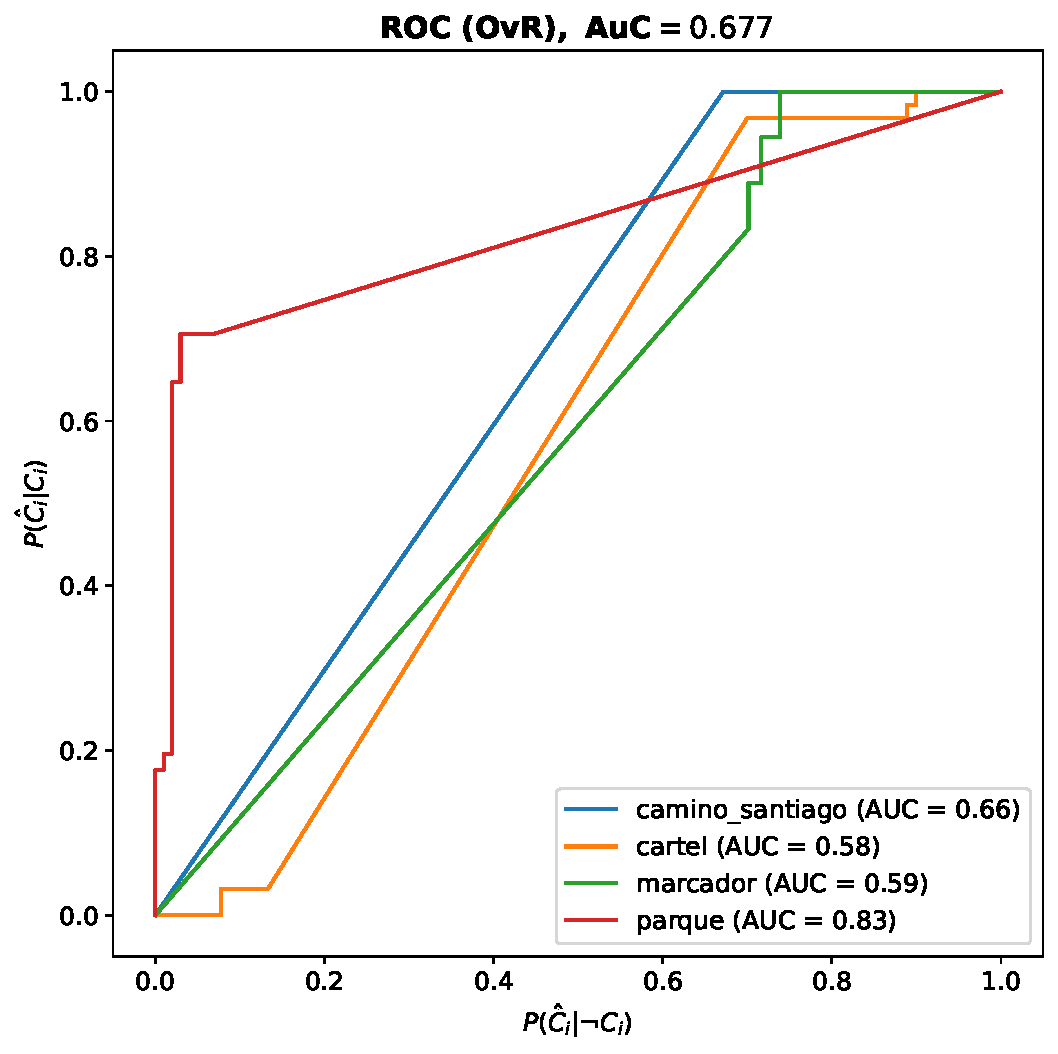
\includegraphics[scale = .5]{auc_conv}
						\caption{Normal}
						\label{fig:roc_conv}
					\end{subfigure}\hfill
					\begin{subfigure}{.4\textwidth}
						\centering
						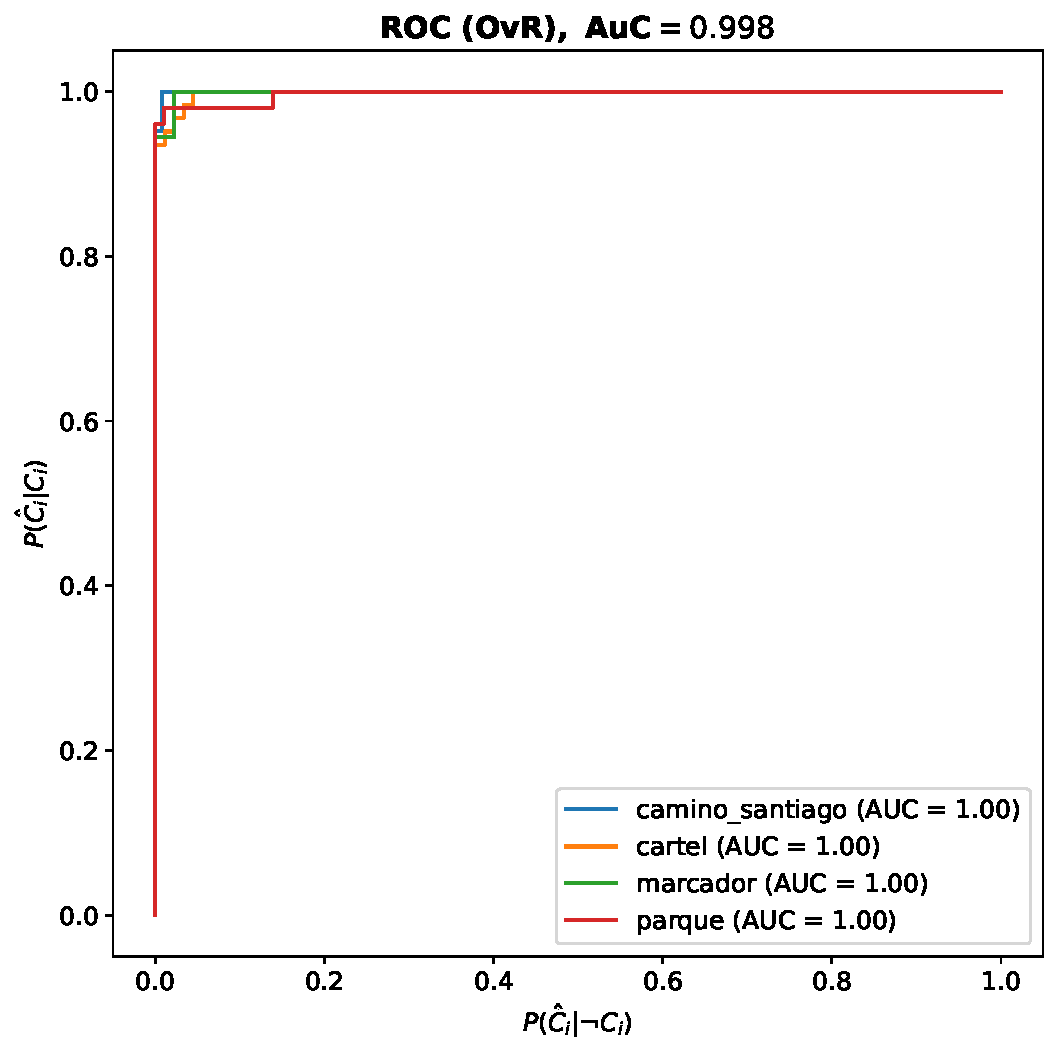
\includegraphics[scale = .5]{auc_mb}
						\caption{Aplicando transfer learning}
						\label{fig:roc_mb}
					\end{subfigure}
					\begin{subfigure}{.4\textwidth}
						\centering
						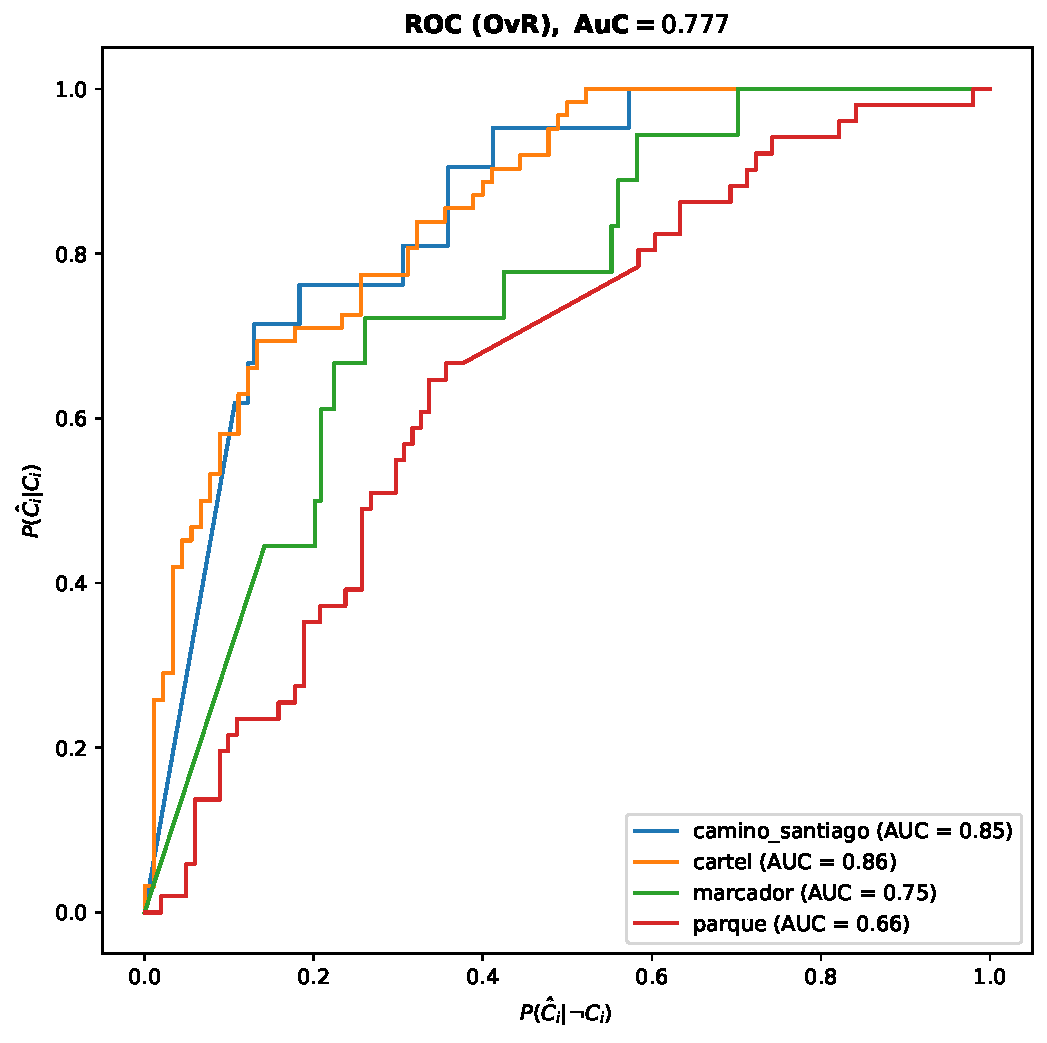
\includegraphics[scale = .5]{auc_convau}
						\caption{Aplicando aumento de datos}
						\label{fig:roc_convau}
					\end{subfigure}\hfill
					\begin{subfigure}{.4\textwidth}
						\centering
						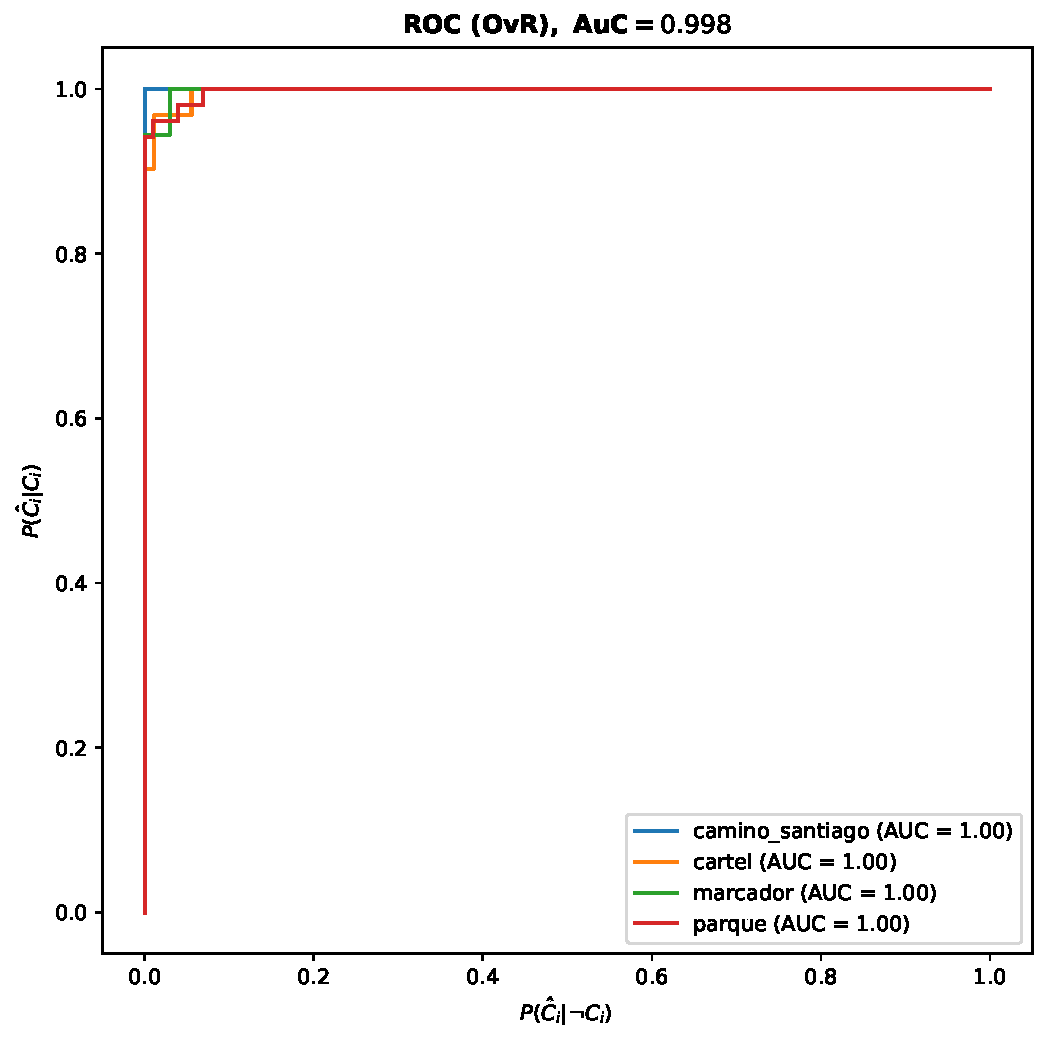
\includegraphics[scale = .5]{auc_mbau}
						\caption{Aplicando ambas}
						\label{fig:roc_mbau}
					\end{subfigure}
					\caption{Curvas ROC}
					\label{fig:roc}
				\end{figure}
			
				Como resumen de esta parte, se puede concluir que el entrenamiento de una red convolucional desde cero es un proceso complejo y que requiere de una cantidad enorme de datos, que en los casos en los que no se dispone de ellos, conduce a resultados negativos, siendo necesario aplicar la técnica de transfer learning. A pesar de haber visto su gran eficacia, se va a realizar una prueba más. \\
				
				El dataset empleado, contenía imágenes de diferentes partes de España, por lo que el modelo estaba viendo variantes de cada tipo de objeto. Lo que se va a hacer ahora es separar dicho dataset de manera que contenga únicamente en el conjunto de test imágenes de la ciudad de Guadalajara. Al ser pocas, el experimento no será muy representativo, pero permitirá probar la eficacia de la red generalizando conceptos. Para ello se ha utilizado el mismo modelo que se ha utilizado en el caso de transfer learning (entrenando de nuevo los parámetros desde cero para evitar hacer predicciones de una imagen vista durante el entrenamiento). \\
				
				\begin{figure}[!h]
					\centering
					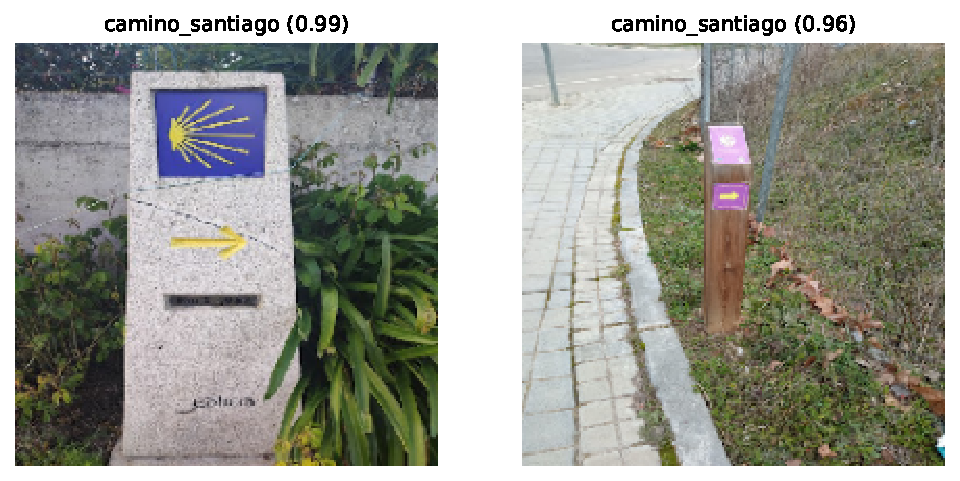
\includegraphics[scale = .8]{gu_vs_ga}
					\caption{Experimento de la capacidad de generalización de la red}
					\label{fig:comparativa_gu}
				\end{figure}
				
				Como se observa en la \Cref{fig:comparativa_gu}, tras haber entrenado el modelo sin usar imágenes de objetos de Guadalajara, y enseñarle uno como por ejemplo este hito del Camino de Santiago, la red está casi segura que de uno de ellos se trata, a pesar de que sea completamente distinto a los que ha visto durante el entrenamiento con el aspecto típico de Galicia. 